\chapter{TOWARDS HIGH DIMENSION}
\label{chap:highdor}
\ifpdf
    \graphicspath{{BipedWalk/HiDofFigs/PNG/}{HiDof/HiDofFigs/PDF/}{HiDof/HiDofFigs/}}
\else
    \graphicspath{{HiDof/HiDofFigs/EPS/}{HiDof/HiDofFigs/}}
\fi
\section{Introduction}
\subsection*{Passivity}
High DOF is key challenging in motion synthesis.
In our research, we partly solved the problem.
For our walking model, when it walk down the slop, all the dof is uncontrolled.
how many dof the walker have doesn't matter.
Even controlled with neural oscilator, only one dof is controlled, 
Even when transformation controller is added, all the dof are controlled, but the matter will not result in underminiestic problem.
For our model, even the dof is not os huge, we have solved extra dof problem completely.

the question arise for model of high degree system, the question is whether the method we developed is applicable for large dof characters.


for our walking and stance example, the question is how the torso should be added, the foot, the side sway and yaw motion, and for system like fish and snake and worm,
they have infinate number dof 

our idea is for different model, 
we should take different measures, 
\begin{itemize}

\HiItem{Neglectable}
for some dof can be neglected for they will have little effects on the qualitative property, 
we can simulate them a different mechanical model, our motion control method don't have to be changed.
because the qualtative property and symmetry is kept.
\HiItem{Symmetry Reduction}
For some DOF,like rotation or pos, the extra dof will have not effects on the dof or the effects can be transformed the dynamic system into transformed version of the orignial system,such Dofs can be reduced.
\HiItem{Mechanical Coupling}
For some high dof system, we can treat them like a coupled mechanical oscillaor, the can only focus on one oscilator.
\HiItem{mimic}
all the three method above are based the effects of dof are not equal, for system that all the dofs are the some, such method will not work.
For dof with similar effects, we can propose a different method, the system is divided into several equal component,we only caculate one component, other mimic the strategy of one.
\end{itemize} 

\section{neglectable}
Although bioliogical mechanical structure is of high degree of freedom, many dof will not have effects on the topology or symmetrical properties.
For the walking example,marcke raiber\citet{Raibert1986} point out walking is the same as a ball rolling down a slope while running is ball bounding down a slope.


we can have system from low dof to high dof as the following picture.
\begin{itemize}
\HiItem{Rimless Wheel}
\HiItem{Compass Gait}
\HiItem{Arch Foot}
\HiItem{Our Model}
\end{itemize}


\begin{figure}[!htbp]
  \begin{center}
    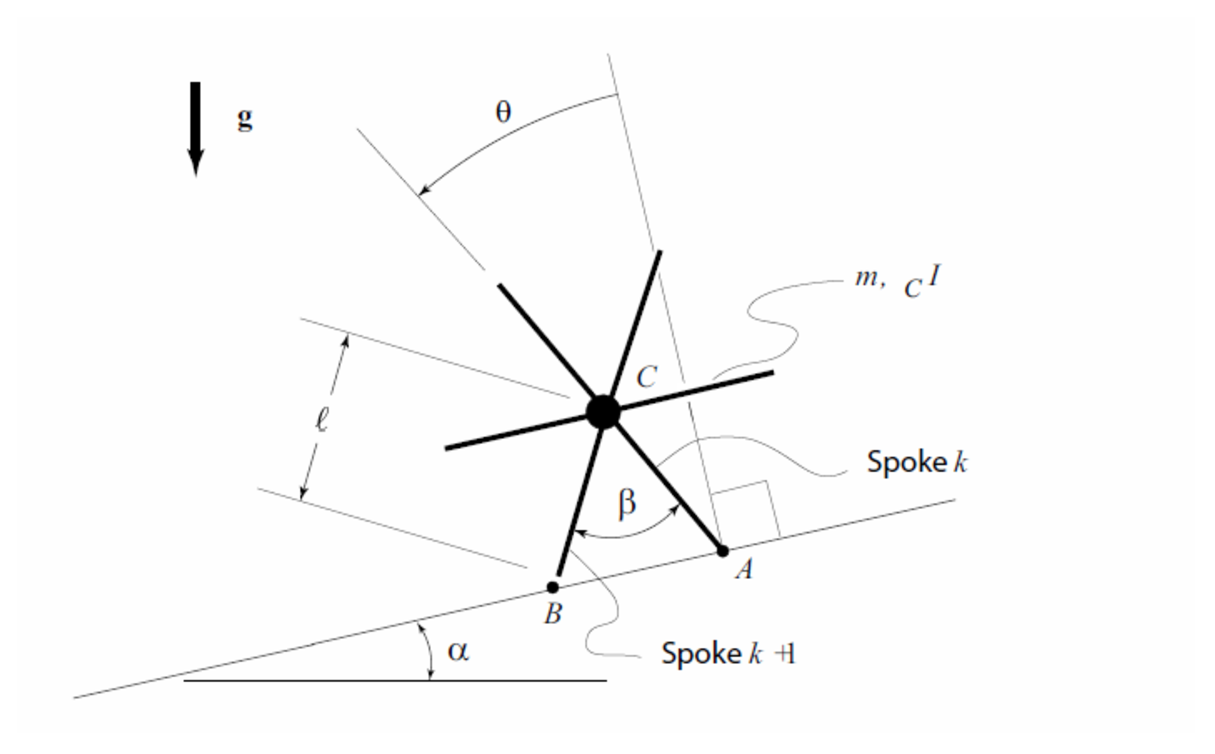
\includegraphics[width=0.7\textwidth]{rimlesswheel}
    \caption{Rimless Wheel}
    \label{fig:rimlesswheel}
\end{center}
\end{figure}


\begin{figure}[!htbp]
  \begin{center}
      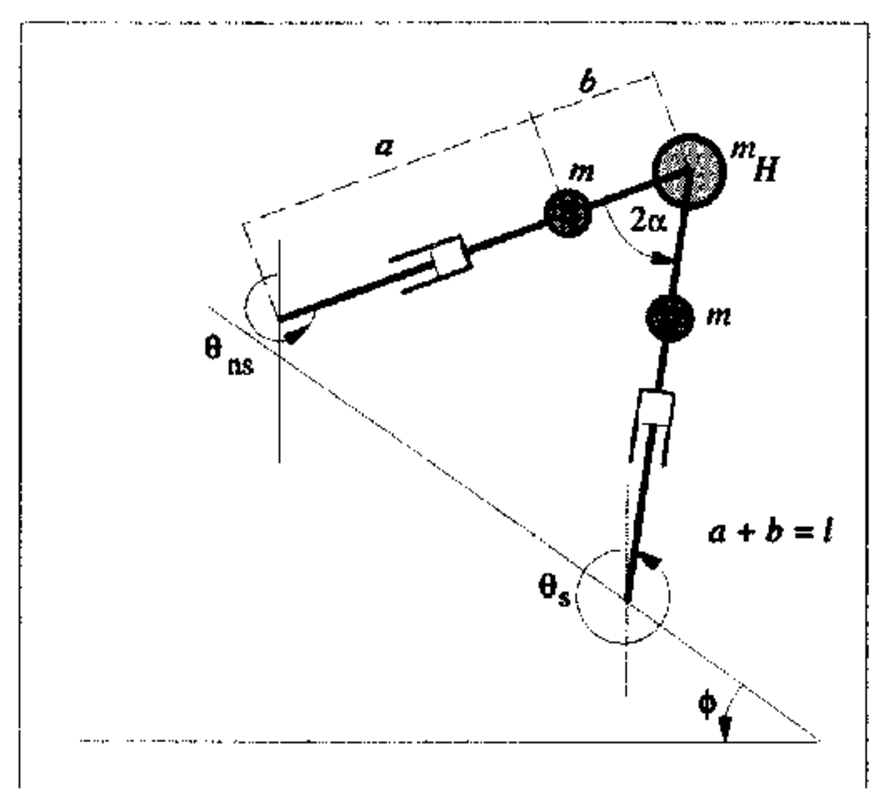
\includegraphics[width=0.7\textwidth]{compassgait}
    \caption{Compass Gait}
    \label{fig:compassgait}
\end{center}
\end{figure}


\begin{figure}[!htbp]
  \begin{center}
      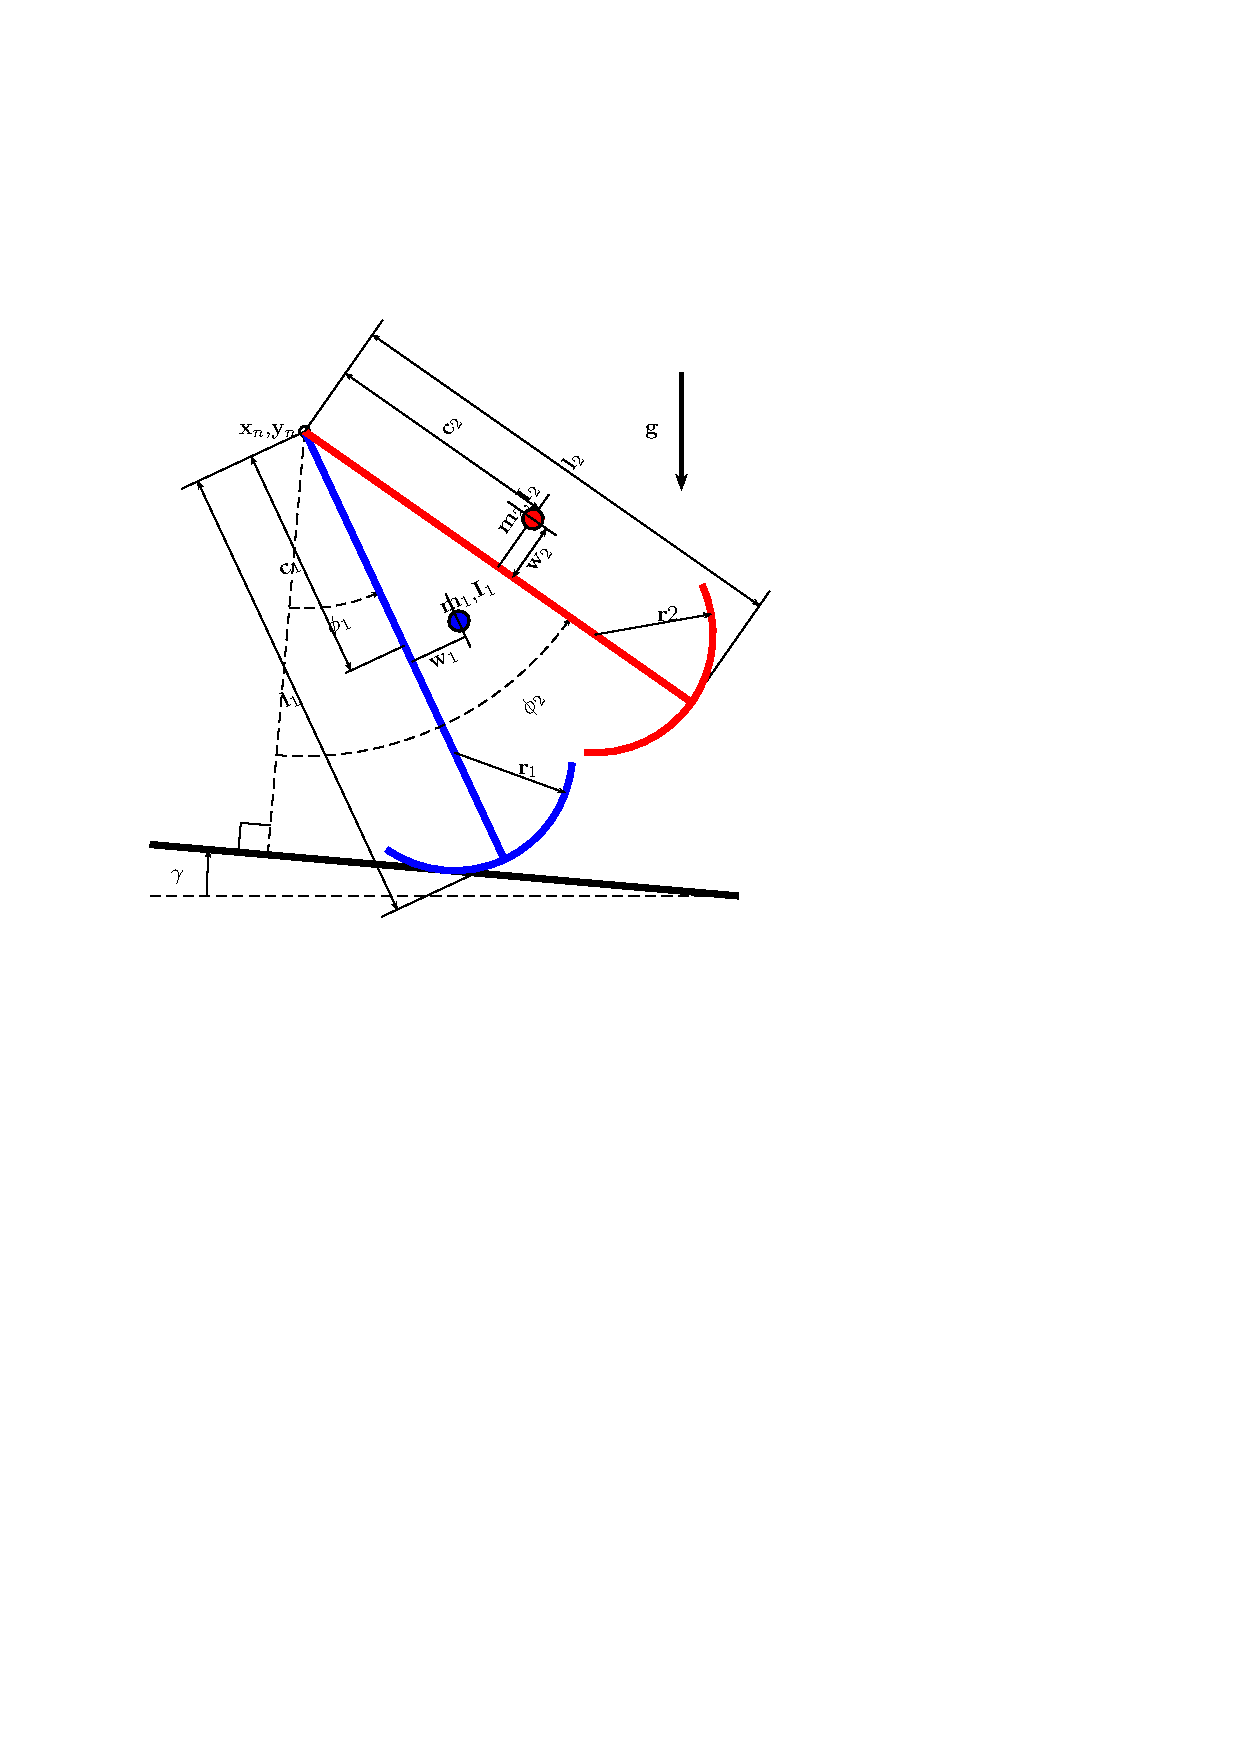
\includegraphics[width=0.7\textwidth]{rollfoot}
    \caption{Compass Gait}
    \label{fig:compassgait}
\end{center}
\end{figure}


compare with our knee walker, all the four models are different but they share the same topology structure and the following three the limit circle shape are very similar.
Thus we can say, the include or knee will not affect the qualitative properties.


And all the four system, can apply the same kind of symmetry group.


This idea may be understand through the perturbation or averaging theory.

In therory all the manifolds share the shape of torus.

if the motion is relatively small,

the dynamics can be approximate as a low dimentional cycle.

as show in Figure.

\begin{figure}[!htbp]
  \begin{center}
      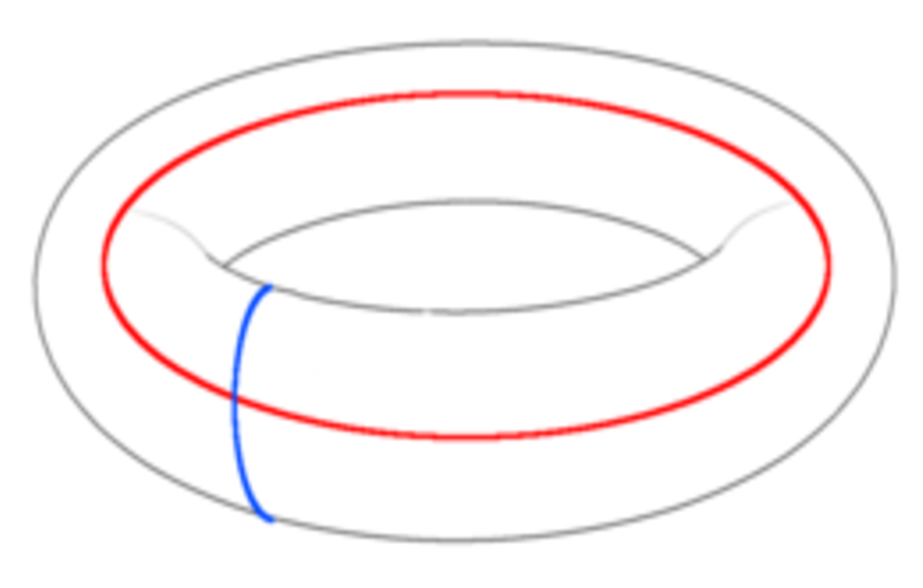
\includegraphics[width=0.7\textwidth]{Torus}
    \caption{Approximate with Torus with a Circle}
    \label{fig:approximate}
\end{center}
\end{figure}


Folowing this idea, although not implemeted in this research, more dofs like foot may also possible.
But that's just an extra level of complexity, without modifying the prinicples. 
\section{Symmetry Reduction}
Some dof will result in a different motion, but such kind of motion will have not qulatitavie effects.
An example is the side sway motion.

the side and front plane is how in picuture.
The side sway effects can be seen can be decoupled for spaghettal function.


For different rotation, will not affect the dynamics on the sphatetal plane.
thus can be neglected.

This method is we can project the gravity in the spagetta plane,
then we see, the way function is just an uniform of minimizing the gravity,
which is the same as speed action.

\begin{figure}[!htbp]
  \begin{center}
      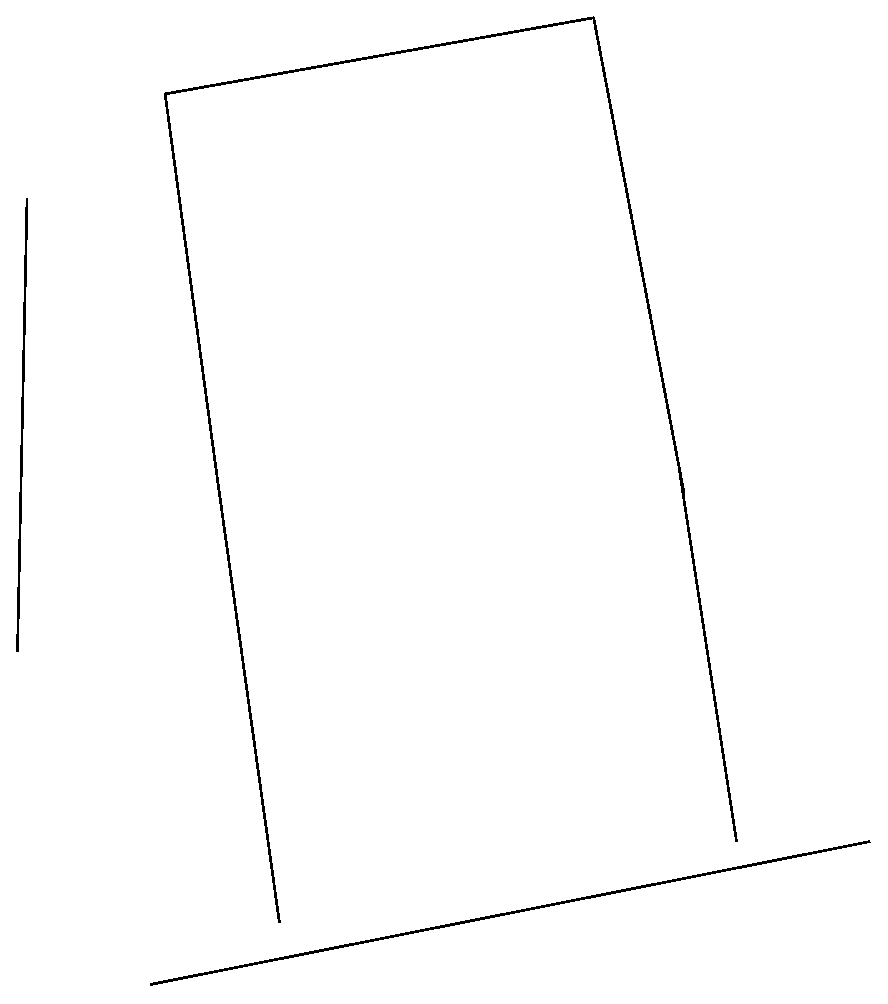
\includegraphics[width=0.7\textwidth]{Sidesway}
    \caption{Sideway}
    \label{fig:sidesway}
\end{center}
\end{figure}


we can project the sideway effects on the sphettal plane. the force is $N'=cos(\alpha)N$
this will the same as appling Speedacition.
With lie group operator such dof can be totally ignored.

\section{Coupled Network}
Some mechanical system can be treated as connecting many different simple components together.
the different parts of motion formed mechanical entrainment.

\subsection*{Mechanical Coupling}
In fact any mechanical system can be treated in this way,
a proper method should separate different components when the coupling is weak.
the weak couple joint can be found through the mechnaical strucutre.

when have mechanical structure in figure
\begin{figure}[!htbp]
  \begin{center}
      \includegraphics[width=0.5\textwidth]{multilink}
    \caption{brances mechanical structure}
    \label{fig:branches structure}
\end{center}
\end{figure}

orignal dynamic system shoud be of 6 DOF and develop the full dynamci system should be of 6 by 6 matrix.
but the matrix will be sparse and their are lots zeros in the $M$ and $C$ matrix.






They happens when they the mechanical have a branch structure.
when mechanical have a branch strucutre,
the dynamic equation will be in the following manner.


based on where the mechanical branches, we can seperate the dynamic equation into two parts,
and simulate them idependently and form the mechanical entrainment network.


if we consider the difference in heel strike phase,
the limit circle becomes more a bit noisy, but qualitative properties are maintained.



\subsection*{Torsol And Arm}
using this method, we can incoroporate the arm and torso motion is our dynamic system.

A without developing the full body dynamic, we can seperate it into two parts.

the torso dynamcis.

the entrainment or torsoq.


by analysizing the equation,
we have find that torso is unstable in nature,
some control effort must be added.
While we know little about it,
in our research, we use a simple pd controller.


through the anaylis ,we know that the torso have little effects on the lower body motion,
that may be why we can carry out many upper body motion while maintain our walk.

It is also possible to use an hybrid method,
we can incoporate motion capture data for the upper body, and adding the effects motion to the lower body.


\section{Boid and Adhoc}

For some sepere and fish, the mechanical system is in chain and involves lots of similar joints.
such system dof can't be neglected or reduced through symmetry and through mechanical coupling.

our propose idea is an adhoc method, we simulate just one dof, other dof following the solution.
since the dynamics is similar, similar strategy will result in similar solution.
such idea have two kinds of application.


The first idea is applying this method for the boid system.
Original boid system are ruled based, but method don't promise stability.
While we useing group theory for simulation boid system, if all the agent using the same neural oscilator, they will converge to the same limit circle,
thus garanty the final motion of the group are in an uniform manner, the different in the agent of modeled by lie group symmetry, different symmetry applied to different agent will result in
difference.
on import symmetry is time offset, which will result in the same motion but of different phases.


In the following example, we have 8 ajent,
the form are controlled by the CPG with the same parameters but of different initiial condition,
this will result an motion of different phase .


we expend this boid example to model the fish swining.
The fish is made up 8 links, and each dof is controllerd by a neural oscillator.

\begin{figure}[!htbp]
  \begin{center}
      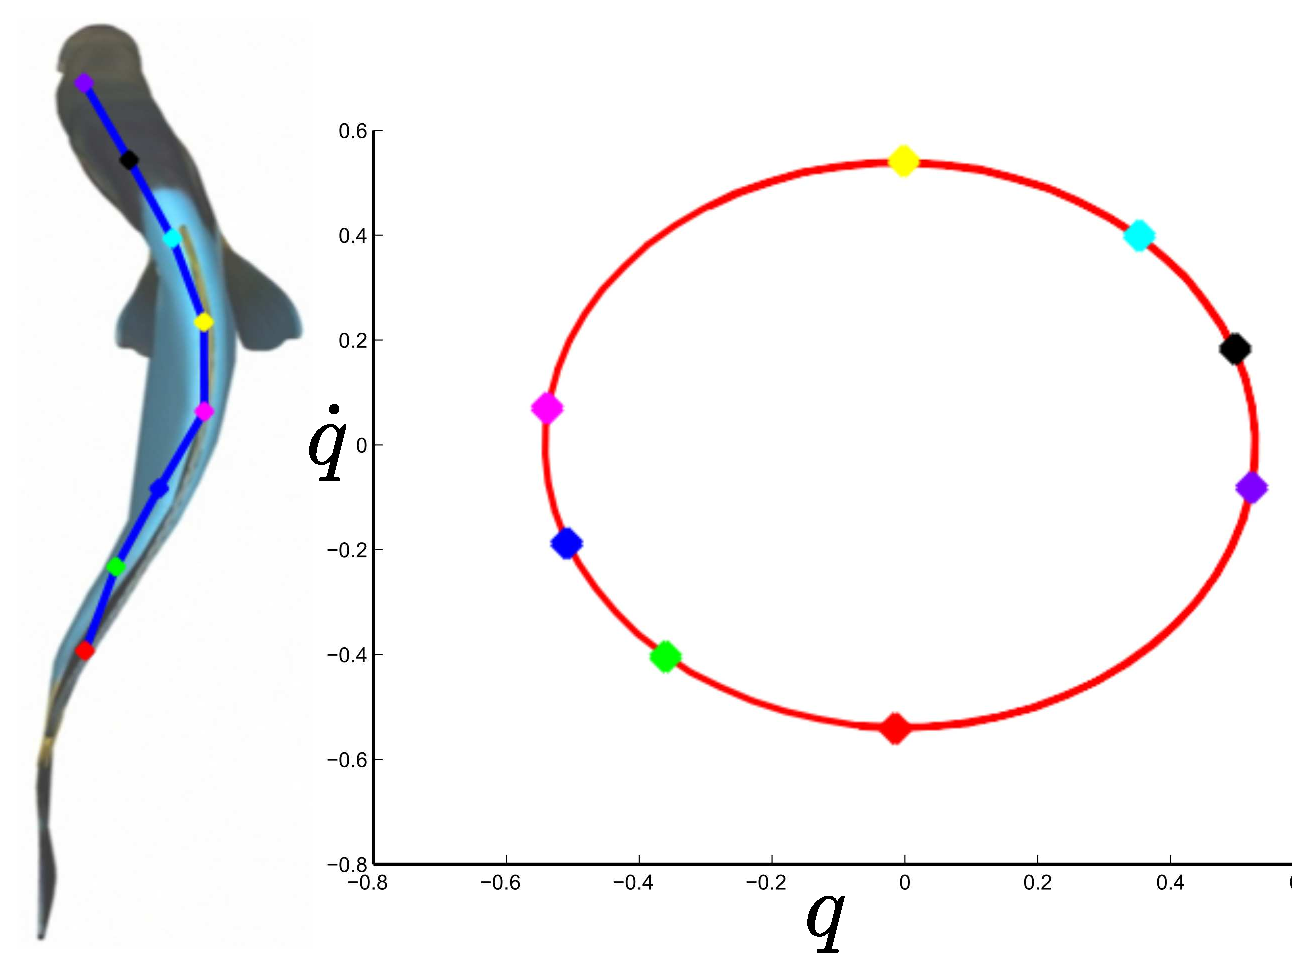
\includegraphics[width=0.5\textwidth]{fish_plot}
    \caption{CPG for Fish}
    \label{fig:fishplot}
\end{center}
\end{figure}

\begin{figure}[!htbp]
  \begin{center}
      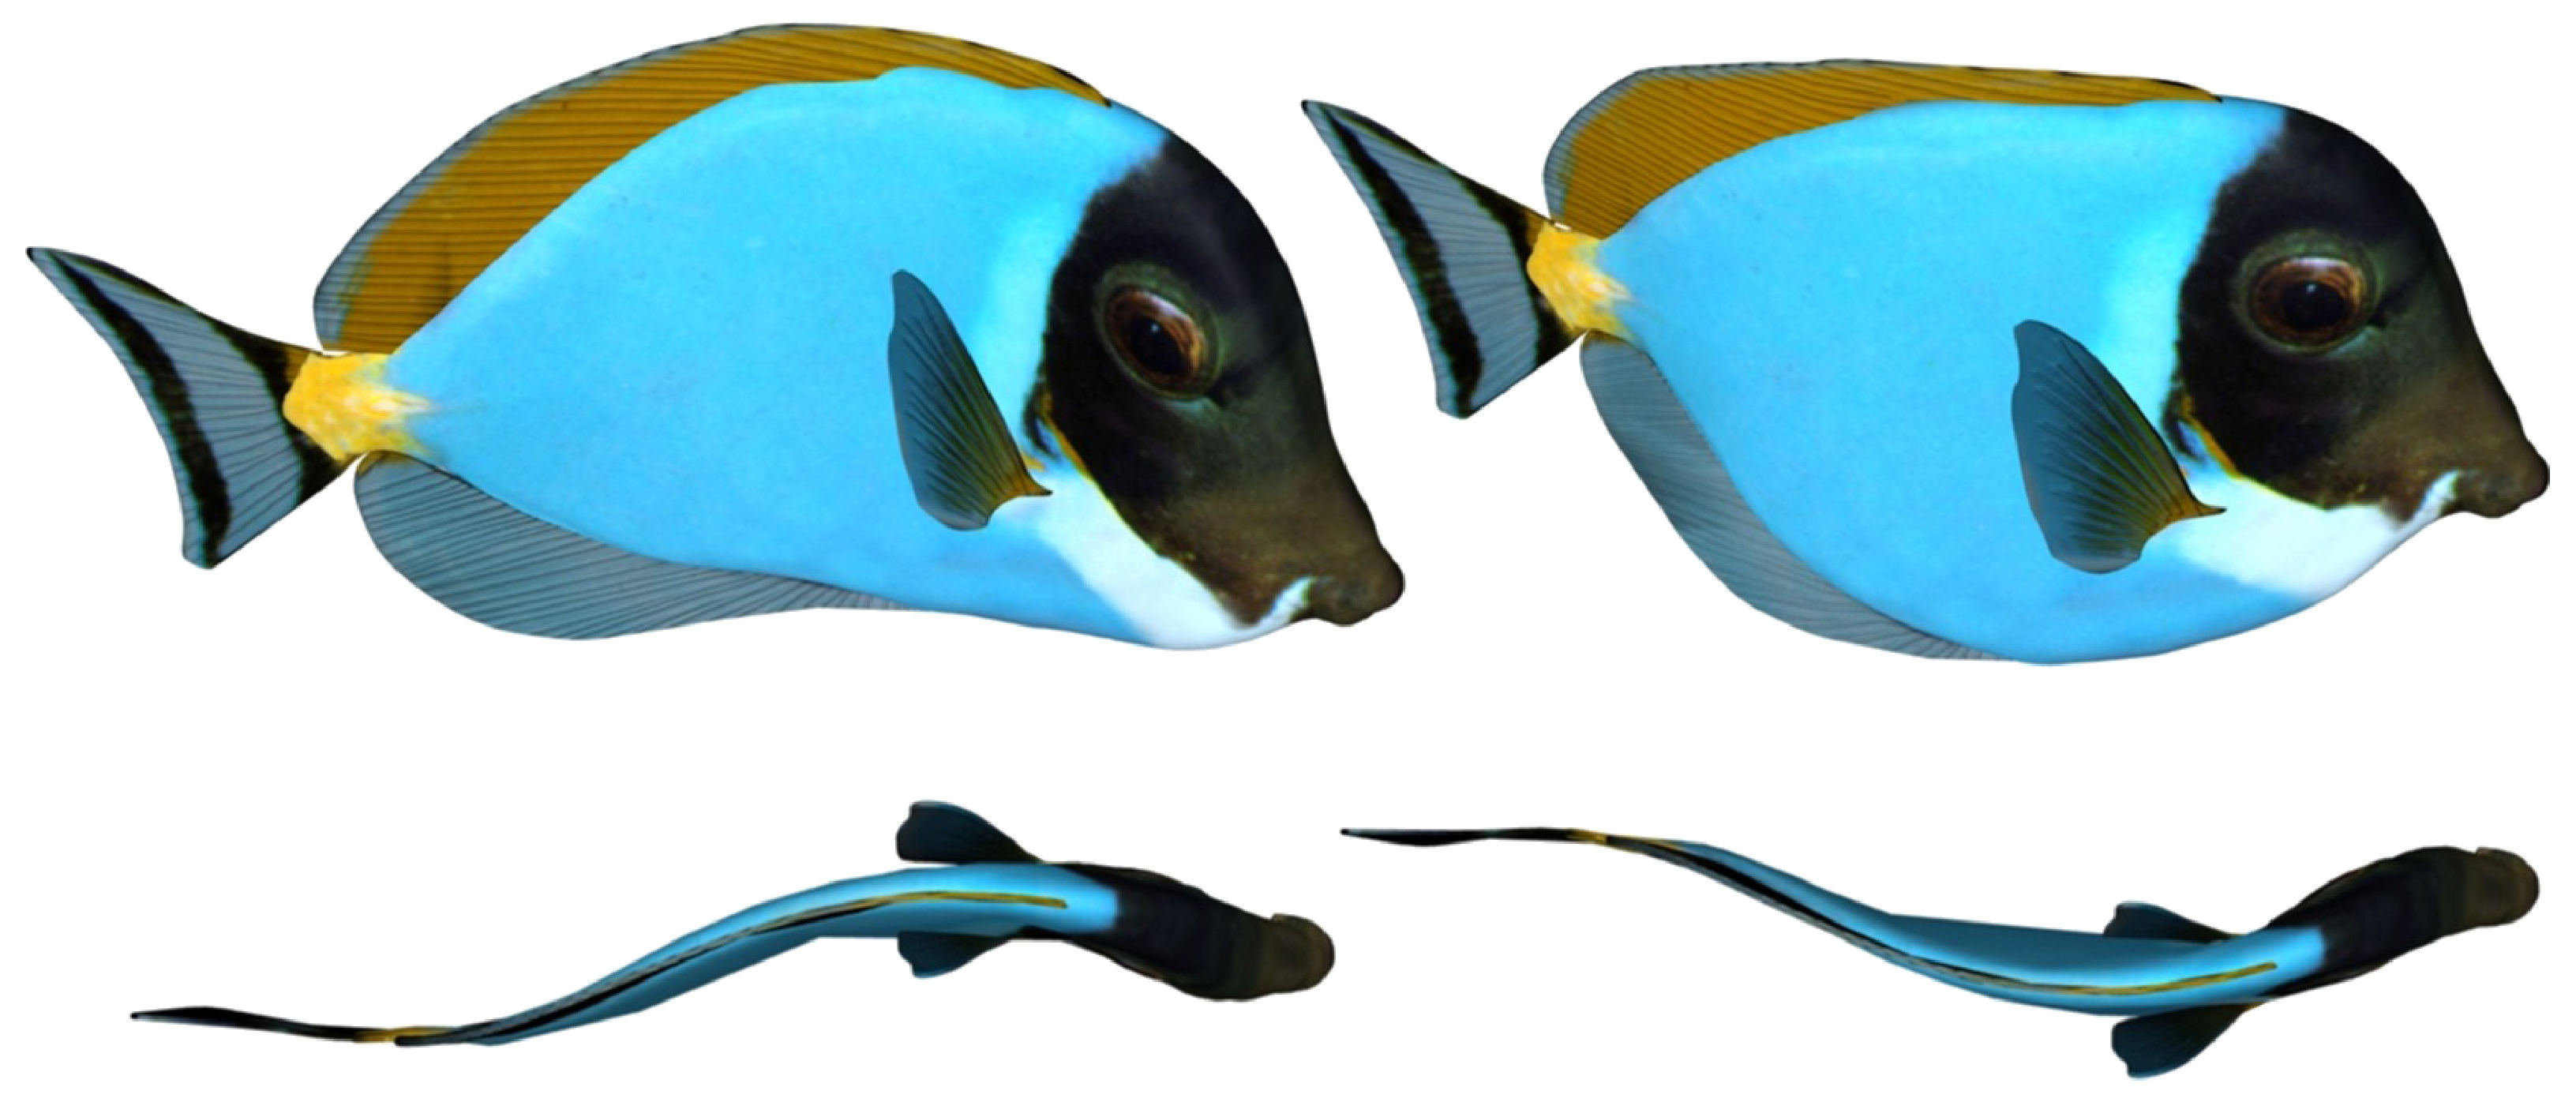
\includegraphics[width=0.5\textwidth]{fish_swimming}
    \caption{Swimming Motion by our method}
    \label{fig:fishswimming}
\end{center}
\end{figure}




the same symmetry is applied to the 8 neural socilator, then it will modify the system in an unified manner.

as show in picture



\section{From Low Dimention To High Dimension}

For computer animation, even we can get high dimentional results, maybe it does not meet the animators needs.
simulation result in motion can be treat as a reference, rather than put into result in deformaiton.

we can discribe the motion procecures, and using mechanical simulation a low dof to drive the high dimensional motion.
in the following exmaple,
we describe the jumping motion in an procedure method,
and bouncing ball is used to drive the motion.


also we can using the low dimension data as a key word to search motion capture data.
which will give us more realistic motion results.


